\section{Experiments}
\label{sec:exp}

We ask five questions.
(1) How many LLM calls does \sys{} need to certify decision queries, compared with existing certified methods and with uncertified sampling?
(2) Do saved calls become saved time when the LLM runs in the loop?
(3) Which of its ingredients produce the savings?
(4) How do proxy quality, the indifference margin, the error level, and the number of groups change the cost?
(5) Does the guarantee hold in practice, including with a misleading proxy?

\subsection{Setup}
\label{sec:setup}

\paragraph*{Datasets}
\textbf{AMZ-Stars} contains 6.84 million reviews from eight categories of the Amazon Reviews 2023 corpus~\cite{amazon2023}.
Its expensive attributes are derived from star ratings and play the role of an LLM judge whose answers are known for every tuple: \textsc{Neg} (1--2 stars), \textsc{Pos} (5 stars), and \textsc{Rating} (1--5).
This lets us vary group structure at scale.
We group reviews by category (8 groups), by year (19 groups), and by product for the two largest categories (the 10 and 30 products with at least 2{,}000 reviews).
\textbf{AMZ-LLM} contains 122{,}251 reviews of 34 products from two categories that AMZ-Stars does not use (video games and musical instruments), namely the products with 1{,}000 to 4{,}000 reviews.
Every review was judged by Qwen2.5-1.5B-Instruct~\cite{qwen25} with three zero-shot prompts: \textsc{Defect} (does the reviewer report a defective, broken, or damaged product?), \textsc{Value} (does the reviewer comment on price or value?), and \textsc{Sent} (overall sentiment on a 1--5 scale).
Neither predicate can be read off the star rating.
We group AMZ-LLM by product within each category (16 and 18 groups) and by year (12 groups).
\textbf{ArXiv-LLM} contains the titles and abstracts of the 309{,}370 papers with a primary computer-science category submitted to arXiv from 2010 to 2021, taken from a public 2021 snapshot of the arXiv metadata~\cite{arxivdata}, and judged by the same LLM with two zero-shot prompts: \textsc{Sota} (does the abstract claim to outperform existing methods or to reach the state of the art?) and \textsc{Emp} (does it report experiments or an empirical evaluation?).
We group the papers by submission year (12 groups of 6{,}409 to 60{,}414) and by primary area (the 16 largest areas, 5{,}057 to 51{,}474 papers), so that real LLM judgments meet large groups.

\paragraph*{Proxies}
Proxies are logistic-regression (binary) or ridge-regression (scores) models on hashed TF-IDF unigrams and bigrams, trained on a labeled set that is disjoint from the queried tuples: 5{,}000 reviews for AMZ-Stars, 3{,}000 LLM-judged reviews for AMZ-LLM, and 3{,}000 LLM-judged abstracts for ArXiv-LLM.
Scoring all 6.8 million AMZ-Stars reviews took about five minutes on one CPU core.
The 3{,}000 LLM judgments that train a proxy cost 2.5\% of a full pass over an AMZ-LLM predicate and 1.0\% over an ArXiv-LLM predicate, once, and are shared by every query over that predicate.
On the queried tuples, the proxies reach AUC 0.960 (\textsc{Neg}) and 0.927 (\textsc{Pos}) and correlation 0.78 (\textsc{Rating}) on AMZ-Stars, AUC 0.963 (\textsc{Defect}) and 0.947 (\textsc{Value}) and correlation 0.79 (\textsc{Sent}) on AMZ-LLM, and AUC 0.923 (\textsc{Sota}) and 0.941 (\textsc{Emp}) on ArXiv-LLM.
The LLM flagged 12.5\% of the reviews as reporting a defect and 20.9\% as commenting on value, and 45.9\% of the abstracts as claiming to beat the state of the art and 59.6\% as reporting experiments.
The weight $\beta$ is estimated by five-fold cross-validation on the labeled set.

\paragraph*{Queries}
For every grouping and attribute we pose a HAVING query with the threshold at the overall mean, an ORDER BY query, and a Top-$k$ query ($k=3$ for eight groups and $k=5$ otherwise), with margin $r$ equal to 5\% of the overall mean and $\alpha=0.05$.
This gives 36 queries on AMZ-Stars, 27 on AMZ-LLM, and 12 on ArXiv-LLM.
Thresholds at the overall mean place several groups close to the boundary, which makes these queries hard for every method.

\paragraph*{Methods}
All methods sample groups without replacement in batches of 100 LLM calls, check their stopping rule after every batch, and use the same decision compilation (\Cref{sec:processing}).
\emph{CLT} and \emph{CLT+P} stop when normal-approximation intervals with finite-population correction (on $y$ and on rectified $z$) separate; they are not certified and serve as the cost floor.
\emph{IFOCUS-HS} uses Hoeffding--Serfling intervals~\cite{hoeffding1963,serfling1974} with a union bound over checks, as in IFOCUS~\cite{ifocus}.
\emph{BlazeIt-EBS} uses the proxy as a control variate and stops with an empirical Bernstein bound and a union bound over doubling checks~\cite{blazeit,mnih2008,maurer2009}.
\emph{Evergreen-CS} uses the without-replacement confidence sequence of Waudby-Smith and Ramdas~\cite{wsr2020wor,wsr2024betting}, the family Evergreen uses for its estimates~\cite{evergreen}, in its closed-form predictable plug-in variant. On the 12 AMZ-Stars HAVING queries, the hedged-capital variant used 0.96--1.26 times its calls (geometric mean 1.06), so we use the stronger closed form throughout. \emph{Evergreen-CS+P} runs the same sequence on rectified values.
\emph{\sys{}} is our method, and \emph{\sys{}--P} is \sys{} without the proxy ($\beta=0$).
Interval methods decide a pair by comparing intervals and use per-group levels $\alpha/K$, so that all intervals hold simultaneously.
Every method samples a group until its decisions are certified or all of its tuples have been judged.
For the \numNQ-query comparison, we judged every tuple once in advance and let each method read these fixed judgments as it samples (\Cref{sec:problem}), making thousands of executions affordable.
\Cref{sec:live} measures all three query forms with two model families issuing fresh LLM calls.

\paragraph*{Implementation and artifacts}
\sys{} and all baselines are implemented in Python with NumPy and share the sampling, batching, and decision code.
The supplementary reproducibility package\footnote{\url{https://github.com/bianyanbo44-afk/VILLE-ICDE2027/releases/tag/v2026.11.11}} contains the code, fixed LLM judgments, proxy scores, result summaries, and per-execution records needed to reconstruct the main comparisons and sensitivity studies.
Cached replays and live runs use the same round scheduler, and the package records every execution's per-round prefixes.

\paragraph*{Metrics}
Cost is the number of LLM calls divided by the number of tuples in the queried groups, averaged over 30 independent runs per query (10 in the sensitivity studies).
The cost of \sys{} varies moderately between runs (coefficient of variation over the 30 runs: median \numCVMED\%, maximum \numCVMAX\% across queries), so each reported average has a relative standard error of at most \numCVSEMAX\%.
Answer error is the fraction of runs whose returned result fails \Cref{def:rcorrect}.
We separately record decision error when a group or a pair used by the answer, at least $r$ from its boundary, is certified on the wrong side or as indifferent.

\subsection{LLM calls to certify a decision}
\label{sec:main}

\begin{table*}[t]
\centering
\caption{LLM calls relative to \sys{}: geometric mean over queries of each method's calls divided by \sys{}'s calls ($>1$: more calls than \sys{}). The \sys{} column gives the median over queries of the fraction of tuples it judged; CLT+P is uncertified.}
\label{tab:main}
\setlength{\tabcolsep}{3pt}
\footnotesize
\begin{tabular}{llrrrrrrrr}
\toprule
Data & Query & $n$ & \sys{} & Everg. & Everg.+P & BlazeIt & IFOCUS & \sys{}$-$P & CLT+P \\
\midrule
AMZ-Stars & HAVING & 12 & 4.6\% & 2.8$\times$ & 1.5$\times$ & 4.7$\times$ & 4.0$\times$ & 1.8$\times$ & 0.55$\times$ \\
 & ORDER BY & 12 & 21.2\% & 2.9$\times$ & 1.7$\times$ & 2.7$\times$ & 3.3$\times$ & 1.6$\times$ & 0.82$\times$ \\
 & Top-$k$ & 12 & 8.4\% & 3.0$\times$ & 1.7$\times$ & 3.8$\times$ & 3.9$\times$ & 1.5$\times$ & 0.76$\times$ \\
\midrule
AMZ-LLM & HAVING & 9 & 19.3\% & 1.8$\times$ & 1.4$\times$ & 3.6$\times$ & 2.4$\times$ & 1.4$\times$ & 0.64$\times$ \\
 & ORDER BY & 9 & 85.6\% & 1.5$\times$ & 1.2$\times$ & 1.6$\times$ & 1.5$\times$ & 1.2$\times$ & 0.83$\times$ \\
 & Top-$k$ & 9 & 23.8\% & 1.9$\times$ & 1.4$\times$ & 3.0$\times$ & 2.3$\times$ & 1.3$\times$ & 0.75$\times$ \\
\midrule
ArXiv-LLM & HAVING & 4 & 2.3\% & 2.3$\times$ & 1.4$\times$ & 4.2$\times$ & 2.0$\times$ & 1.6$\times$ & 0.60$\times$ \\
 & ORDER BY & 4 & 28.1\% & 2.2$\times$ & 1.6$\times$ & 2.7$\times$ & 2.1$\times$ & 1.4$\times$ & 0.79$\times$ \\
 & Top-$k$ & 4 & 2.7\% & 3.0$\times$ & 1.7$\times$ & 4.9$\times$ & 2.8$\times$ & 1.5$\times$ & 0.80$\times$ \\
\midrule
All & & 75 & & 2.3$\times$ & 1.5$\times$ & 3.3$\times$ & 2.8$\times$ & 1.5$\times$ & 0.72$\times$ \\
\bottomrule
\end{tabular}
\end{table*}
\begin{figure*}[t]
\centering
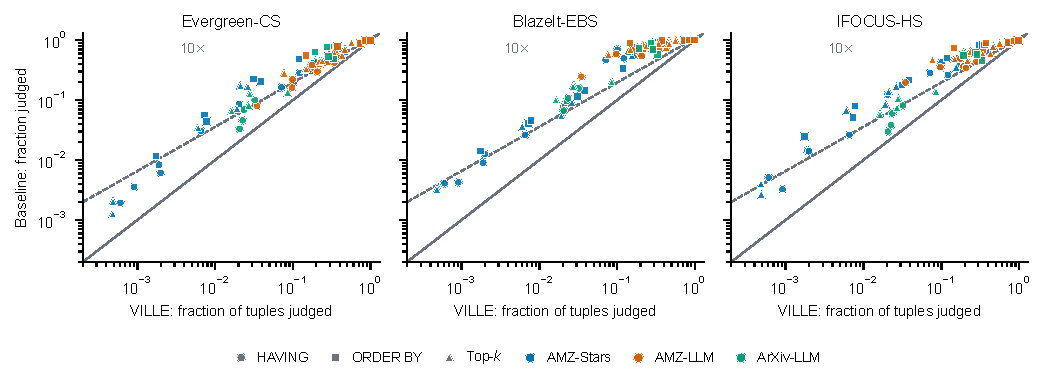
\includegraphics[width=\textwidth]{figures/fig_main_scatter.pdf}
\caption{Fraction of tuples judged per query: \sys{} (x-axis) against each certified baseline (y-axis). Each point is one query (mean over 30 executions); marker shape gives the query type and color the dataset. Points above the solid line cost the baseline more calls than \sys{}; points above the dashed line cost at least ten times more.}
\label{fig:main}
\end{figure*}

\sys{} judged at most as many tuples as Evergreen-CS and BlazeIt-EBS on every one of the \numNQ{} queries, and at most as many as IFOCUS-HS on all but one (\Cref{tab:main} and \Cref{fig:main}).
Across all queries, Evergreen-CS judged \numRWSR$\times$ as many tuples as \sys{} (geometric mean; up to \numRWSRMAX$\times$), BlazeIt-EBS \numRBSP$\times$, and IFOCUS-HS \numRHS$\times$.

The savings grow with group size: across all queries, the saving over Evergreen-CS rises with the mean group size (Spearman $\rho=\numRHOGS$), from \numBINA$\times$ for groups below 5{,}000 tuples to \numBINB$\times$ between 5{,}000 and 50{,}000 and \numBINC$\times$ above.
On ArXiv-LLM, which combines real LLM judgments with groups of 5{,}000 to 60{,}000 abstracts, Evergreen-CS judged \numAXRWSR$\times$ as many tuples as \sys{}, BlazeIt-EBS \numAXRBSP$\times$, and IFOCUS-HS \numAXRHS$\times$; finding the five years with the highest share of abstracts that claim to beat the state of the art took \sys{} 8{,}557 calls and Evergreen-CS 38{,}563.
On the category and year groupings of AMZ-Stars, whose groups hold $10^4$ to $10^6$ reviews, Evergreen-CS judged 4.4$\times$ and 5.2$\times$ as many tuples as \sys{}, and IFOCUS-HS 6.7$\times$ and 6.5$\times$.
For example, \sys{} answered the HAVING query on the share of negative reviews per year with 139{,}097 LLM calls, whereas Evergreen-CS, BlazeIt-EBS, and IFOCUS-HS needed 583{,}720, 434{,}123, and 847{,}783; ranking the 19 years by their share of five-star reviews took \sys{} 213{,}170 calls and Evergreen-CS 1.53 million.
On product groups, which hold one to thirty thousand reviews and often differ by little more than the margin, every certified method judges a large share of each group, and the finite-population form of the tests lets all of them stop once little uncertainty remains.
AMZ-LLM consists only of such groups (1{,}000 to 4{,}000 reviews per product, at most 16{,}704 per year).
There \sys{} judged \numAMZLRWSR$\times$ fewer tuples than Evergreen-CS, \numAMZLRBSP$\times$ fewer than BlazeIt-EBS, and \numAMZLRHS$\times$ fewer than IFOCUS-HS, with the largest gains on the year grouping (1.9$\times$ over Evergreen-CS).

Certification costs no more than common practice.
The usual procedure samples until normal-approximation intervals separate; it carries no guarantee, yet it judged \numRCLT$\times$ as many tuples as \sys{}.
Run on proxy-rectified values (CLT+P), the same procedure judged \numRCLTP$\times$ as many tuples, so \sys{} pays about \numRCLTPINV$\times$ the calls of this uncertified counterpart for a guarantee that holds at every stopping time.
Neither procedure is uncertified merely in principle: on AMZ-LLM, CLT returned an incorrect answer in up to 13\% of a query's executions and CLT+P in up to 7\%, while no certified method erred (\Cref{sec:validity}).
Skipping the LLM altogether is worse still: answering from each group's mean proxy score, which costs no LLM call, gave an answer that is not $r$-correct on \numNPROXYWRONG{} of the \numNPROXYQ{} queries.

\subsection{Live query execution}
\label{sec:live}

We measure how certification translates into query latency with two model families,
Qwen2.5-1.5B-Instruct and SmolLM2-1.7B-Instruct~\cite{smollm2}, on an RTX 4060 laptop GPU (8\,GB).
A DuckDB group-by supplies the product identifiers and row lists of the video-game reviews.
We select a shared workload of \numLiveN{} reviews in 16 products by uniformly sampling at most 2{,}000 evaluation reviews per product.
Selection uses metadata, and each model receives a separate proxy trained on its judgments of the existing disjoint 3{,}000-review training split.
Both models use the \textsc{Defect} prompt and the same query parameters, fixed before the additional judgments are collected.
The HAVING threshold is 0.20, the indifference margin is 0.01, $\alpha=0.05$, and $k=5$.

\begin{table*}[t]
\centering
\caption{Live execution with two model families over the same 32,000 reviews in 16 product groups: latency tracks the number of LLM calls, and certificate updates take at most \numLiveMaxOverhead\% of \sys{}'s latency.
CS denotes the Evergreen-style confidence-sequence baseline. Calls count fresh model evaluations by each method.
Latencies include prompt processing, model inference and certificate updates, with the model
resident and proxies prepared. Each model's complete exact scan is measured once and supplies the shared reference
latency for the three queries over the same predicate. The SQL aggregation time is added per query.
Speedup is measured exact-query latency divided by VILLE latency.}
\label{tab:online}
\footnotesize
\setlength{\tabcolsep}{5pt}
\renewcommand{\arraystretch}{1.12}
\begin{tabular}{llrrrrrr}
\toprule
& & \multicolumn{2}{c}{LLM calls} & \multicolumn{3}{c}{Measured latency (s)} & \\
\cmidrule(lr){3-4}\cmidrule(lr){5-7}
Model & Query & \sys{} & CS & \sys{} & CS & Exact & Speedup \\
\midrule
Qwen2.5-1.5B & HAVING & 12,400 & 15,100 & 229.3 & 280.0 & 570.3 & 2.49$\times$ \\
 & ORDER BY & 26,400 & 30,000 & 484.8 & 558.0 & 570.3 & 1.18$\times$ \\
 & Top-5 & 16,500 & 19,700 & 312.3 & 378.4 & 570.3 & 1.83$\times$ \\
\midrule
SmolLM2-1.7B & HAVING & 1,900 & 2,000 & 44.6 & 47.9 & 712.8 & 15.97$\times$ \\
 & ORDER BY & 32,000 & 31,500 & 709.2 & 699.6 & 712.8 & 1.00$\times$ \\
 & Top-5 & 23,700 & 25,400 & 515.5 & 556.1 & 712.7 & 1.38$\times$ \\
\bottomrule
\end{tabular}
\end{table*}


\sys{} and Evergreen-CS issue fresh model requests for every query, using the same random group permutations and 100-tuple request blocks.
The decision layer consumes the row lists, updates its certificates, and charges every tuple actually sent to the model.
The table reports one complete execution per configuration with the model resident and proxy scores prepared, following the amortized-proxy setting.
For each model, we also execute a complete scan of all \numLiveN{} reviews.
SQL aggregation of its judgments supplies the reference answers for HAVING, ORDER BY and Top-5.
The measured scan time is their shared exact-evaluation reference, with the SQL aggregation time added per query.

All six \sys{} answers are $r$-correct, and every live judgment agrees with the corresponding model's complete pass (\Cref{tab:online}).
Saved calls became saved time one for one: in all twelve sampled executions, the latency per call stayed within 8\% of that of the model's full scan, and certificate updates and query bookkeeping took at most \numLiveMaxOverhead\% of \sys{}'s latency.
The call counts of \Cref{sec:main} therefore translate directly into latency.
On Qwen2.5, HAVING takes 12{,}400 calls and 229.3\,s against 32{,}000 calls and 570.3\,s for full evaluation, a \numLiveHavingMin$\times$ speedup.
SmolLM2 reports a defect in under 10\% of every product's reviews, far below the threshold, so HAVING is certified after 1{,}900 calls and 44.6\,s against 712.8\,s, a \numLiveHavingMax$\times$ speedup.
With 2{,}000 reviews per product and a margin of one percentage point, ranking all 16 products requires most of each group; the workload isolates how calls convert into latency.

\subsection{Where the savings come from}
\label{sec:ablation}

\begin{figure}[t]
\centering
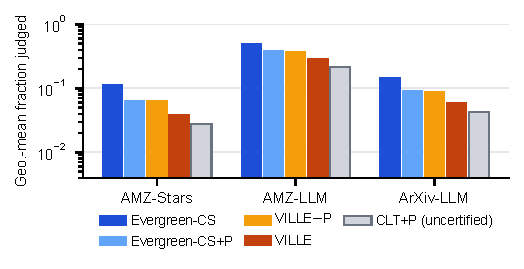
\includegraphics[width=\columnwidth]{figures/fig_decomposition.pdf}
\caption{Where the savings come from. Geometric-mean fraction of tuples judged over the queries of each dataset, for the Evergreen-style confidence sequence with and without the proxy, \sys{} with and without the proxy, and the uncertified CLT+P floor.}
\label{fig:decomp}
\end{figure}

\begin{figure}[t]
\centering
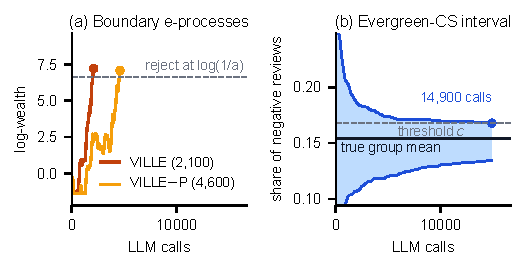
\includegraphics[width=\columnwidth]{figures/fig_anatomy.pdf}
\caption{One HAVING decision on AMZ-Stars: is the share of negative reviews in 2017 (752{,}784 reviews, true share 15.4\%) below the threshold of 16.8\%? (a) Log-wealth of the boundary test with and without the proxy, drawn until it reaches $\log(1/a)$. (b) The Evergreen-style confidence sequence, drawn until its upper bound falls below the threshold. One run; the same tuples are judged in the same order.}
\label{fig:anatomy}
\end{figure}

\Cref{fig:anatomy} dissects a single decision.
The 2017 group lies 1.6$r$ below the threshold.
The confidence sequence must shrink until its upper bound clears the threshold, which takes 14{,}900 calls.
The boundary test only has to accumulate evidence against one value and rejects after 4{,}600 calls without the proxy; betting on rectified values halves this again, to 2{,}100 calls.

Two mechanisms contribute about equally, and their effects multiply (\Cref{fig:decomp}).
Holding the confidence sequence fixed, adding the proxy (Evergreen-CS $\rightarrow$ Evergreen-CS+P) cut LLM calls by \numAMZSPROXYEFF$\times$ on AMZ-Stars, \numAMZLPROXYEFF$\times$ on AMZ-LLM, and \numAXPROXYEFF$\times$ on ArXiv-LLM (geometric means).
Holding the proxy fixed, the gap-adaptive boundary tests and direct paired construction (Evergreen-CS+P $\rightarrow$ \sys{}) cut them by a further \numAMZSBOUNDEFF$\times$, \numAMZLBOUNDEFF$\times$, and \numAXBOUNDEFF$\times$.
Without the proxy, \sys{}$-$P still judged \numAMZSBETVSWSR$\times$, \numAMZLBETVSWSR$\times$, and \numAXBETVSWSR$\times$ fewer tuples than Evergreen-CS, showing the contribution of these betting and paired-test choices.
For orderings, the paired tests add to this, because two confidence sequences must clear the gap together, whereas the paired test pays once for the deviation of the difference.
The proxy also repays its training labels: on the two LLM-judged datasets, \sys{} issued \numPROXYSAVEMIN{} to \numPROXYSAVEMAX{} thousand fewer calls per predicate than \sys{}$-$P over the queries we posed, against the 3{,}000 calls that trained each proxy.

\subsection{Proxy quality, margin, and scale}
\label{sec:sensitivity}

\begin{figure*}[t]
\centering
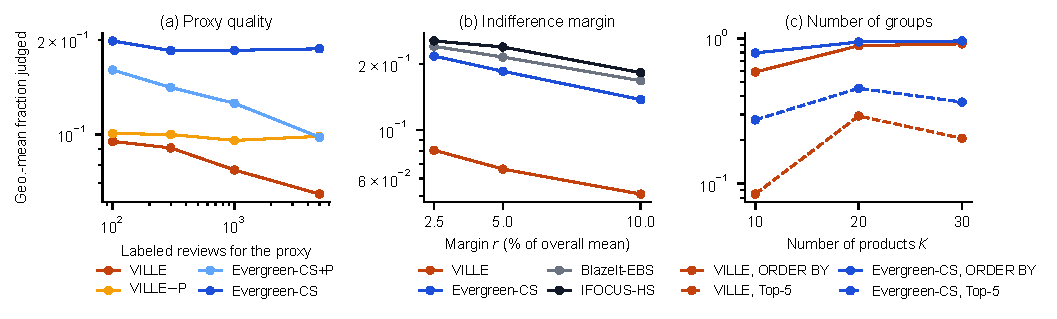
\includegraphics[width=\textwidth]{figures/fig_sensitivity.pdf}
\caption{Sensitivity on AMZ-Stars \textsc{Neg} queries (geometric mean over the year and Appliances-product groupings). (a) Proxies trained on 100 to 5{,}000 labeled reviews. (b) Indifference margin $r$. (c) Number of groups for ORDER BY and Top-5.}
\label{fig:sens}
\end{figure*}

Proxy quality governs the size of the saving, not its sign (\Cref{fig:sens}a).
We retrained the \textsc{Neg} proxy on 1{,}000, 300, and 100 of the 5{,}000 labeled reviews, which lowered its AUC from 0.960 to 0.941, 0.901, and 0.836.
With the weakest proxy, \sys{} judged 6\% fewer tuples than without a proxy; with the strongest, 35\% fewer.
In every case \sys{} stayed below Evergreen-CS, by 2.1$\times$ with the weakest proxy and 2.9$\times$ with the strongest, so even a proxy trained on 100 labels is worth using.

The margin trades precision for calls without changing the comparison (\Cref{fig:sens}b).
Halving $r$ from 5\% to 2.5\% of the overall mean raised \sys{}'s cost by 22\%, and doubling it to 10\% lowered the cost by 23\%; Evergreen-CS judged between 2.7$\times$ and 2.8$\times$ as many tuples at every margin.
The error level matters little, because the cost grows with $\log(1/\alpha)$ (\Cref{eq:cost}): tightening $\alpha$ from 0.05 to 0.01 raised \sys{}'s cost by 15\% and Evergreen-CS's by 13\%, and loosening it to 0.10 lowered both by 5\% to 6\%.

Cost depends on how close the groups are rather than on how many there are (\Cref{fig:sens}c).
Among the Appliances products, adding those ranked 11 to 20 by review count raised every method's cost, whereas adding products 21 to 30 lowered every method's Top-5 cost and changed each certified method's ORDER BY cost by at most 3\%, because the cost of a decision is driven by how close its groups are to each other.
\sys{} judged 1.4$\times$ to 1.9$\times$ fewer tuples than Evergreen-CS at 10, 20, and 30 groups (geometric mean over the three query forms), although the union bound over pairs grows quadratically with the number of groups.

\subsection{Validity}
\label{sec:validity}

\begin{table}[t]
\centering
\caption{Errors over all 75 queries, each executed 30 times. Answer errors violate the returned-result definition of $r$-correctness. Decision errors concern a group or pair used by the answer, at least $r$ from its boundary, certified on the wrong side or as indifferent. The last column is the highest per-query answer-error rate.}
\label{tab:validity}
\footnotesize
\begin{tabular}{lrrr}
\toprule
Method & Answers & Decisions & Worst rate \\
\midrule
\sys{} & 0 / 2250 & 0 / 2250 & 0.00 \\
\sys{}$-$P & 0 / 2250 & 0 / 2250 & 0.00 \\
Evergreen-CS & 0 / 2250 & 0 / 2250 & 0.00 \\
Evergreen-CS+P & 0 / 2250 & 0 / 2250 & 0.00 \\
BlazeIt-EBS & 0 / 2250 & 0 / 2250 & 0.00 \\
IFOCUS-HS & 0 / 2250 & 0 / 2250 & 0.00 \\
CLT (uncert.) & 5 / 2250 & 16 / 2250 & 0.13 \\
CLT+P (uncert.) & 3 / 2250 & 3 / 2250 & 0.07 \\
\bottomrule
\end{tabular}
\end{table}

No certified method returned an incorrect answer in any of the \numNEXEC{} query executions (\Cref{tab:validity}).
Uncertified CLT returned an incorrect answer in \numNCLTERR{} executions spread over \numNCLTERRQ{} queries, and CLT+P in \numNCLTPERR{} executions over \numNCLTPERRQ{} queries; the worst rates, 13\% and 7\%, occurred on AMZ-LLM queries about defects.
The normal approximation errs rarely, but silently: nothing in a single execution reveals when it has failed.
To probe the tests directly, we ran each test 2{,}000 times on finite populations whose mean sits exactly on the null boundary, a Bernoulli population of 20{,}000 tuples and a skewed population of 5{,}000 tuples, with $a=0.05$.
The one-sample tests rejected in 1.4\% to 2.1\% of runs and the paired test, applied to groups of 3{,}000 and 8{,}000 tuples, in 1.1\%, both below the nominal 5\%.

A misleading proxy costs calls but not correctness.
We replaced the \textsc{Neg} proxy on the year grouping by its inversion $1-p$, by uniform noise, and by a random permutation of its scores, and forced $\beta=1$ instead of letting cross-validation shrink it.
\sys{} remained error-free in all 90 executions.
Relative to \sys{}$-$P, its largest cost ratios were 1.71$\times$ with the inverted proxy, 1.55$\times$ with noise, and 1.16$\times$ with the permuted scores. It stayed below Evergreen-CS in every case.
The cross-validated coefficient used elsewhere downweights uninformative proxies toward $\beta=0$ and clips negatively correlated proxies to zero.

\subsection{Scope}
\label{sec:scope}

\sys{} assumes that the LLM judgment of a tuple is fixed once computed, which holds with deterministic decoding and caching, and that tuples are sampled uniformly within each group.
Its guarantee concerns the decisions that the LLM itself would reach on all tuples; the fidelity of the LLM to human judgment is a separate question that applies equally to exact evaluation.
The size of the saving depends on how well the proxy tracks the LLM in use, whereas the guarantee does not.
The union bound over groups and pairs is the simplest way to control all decisions at once.
Because every test produces an e-value, replacing the union bound by e-value-based false discovery rate control~\cite{wang2022ebh} is a direct extension for dashboards with hundreds of groups.
